\subsection{Recovering known structure from simulated populations.}

\begin{figure}
    \centering
    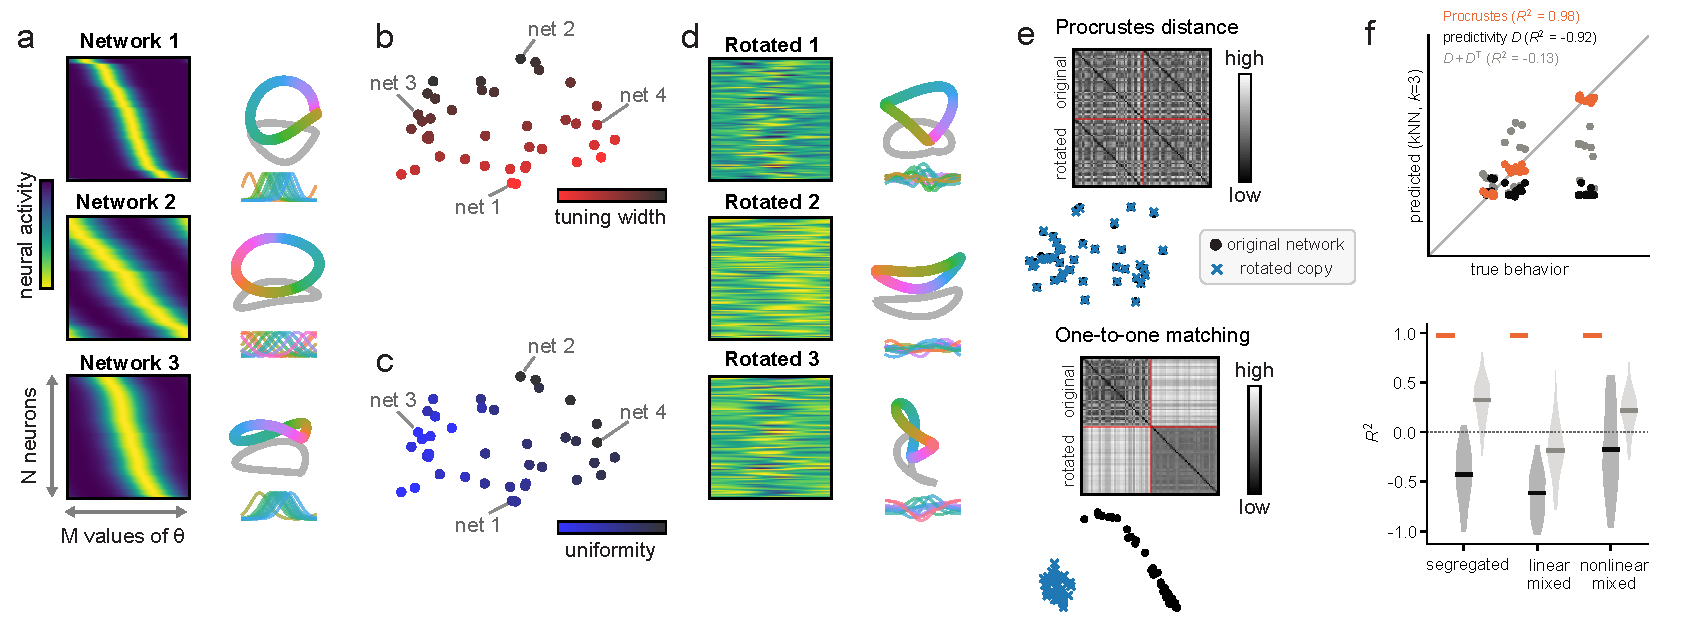
\includegraphics[width=0.95\textwidth]{content/figures/netrep-journal-figure-2b.pdf}
    \caption{\textbf{Metric structure enables behavioral prediction from population geometry in simulated cohorts} \textbf{a.} Left, three example datasets (out of $K = 40$) of $N = 100$ neurons sorted by their preferred stimulus $\theta$, with varying tuning width and concentration of tuning around $\theta = 0$.  Right, first 3 principle components of the same datasets show how tuning curves parameters shape neural manifolds. Inset, example tuning curves highlighting differences in tuning width and uniformity. \textbf{b-c.} Embedding of $K \times K$ matrix dissimilarity matrices in 2D (Methods), shows that the shape metric successfully captured the two forms of across-subject variability, tuning curve width along one dimension (b) and tuning concentration long another (c).  \textbf{d.} Randomly rotated copy of each network in a. \textbf{e.} Top, Similar to b, but done for rotated and original networks in d) and a), respectively. Each neural system and its rotated copy lie on top of each other in the
low-dimensional space, when using Procrustes distance. Bottom, Differences in single-neuron tuning structure in rotated and original networks are are captured by one-to-one matching distance.  \textbf{f.} A separate cohort of $K = 30$ subjects differing in tuning width, which sets acuity, and how many other task variables they encode, which does not sets acuity. \textit{Top}, acuity predicted from each subject's position in the space ($k = 3$ nearest neighbors) under Procrustes distance (orange), linear predictivity (black) and its symmetrized form $(\mbD + \mbD^\top)/2$ (grey). \textit{Bottom}, same comparison across 50 resampled cohorts and three ways of encoding different
  variables (segregated neural populations, linearly mixed, nonlinearly mixed).
% \textbf{h.} Estimating true information of the original networks from 3 nearest neighbors rotated networks is worse when using permutation distance metrics (blue) than Procrustes (black).
}
     \label{fig:synth}
\end{figure}

We now turn to practical demonstrations using simulations, before turning to experimental data.
For simplicity, we simulated data from a population of neurons encoding a periodic variable, $\theta$.
As $\theta$ is varied, the firing rate traces out a smooth, 1D ring manifold in the high-dimensional firing rate space (\textit{Fig.} \ref{fig:schematic}d).
Figure~\ref{fig:synth}a shows tuning curves (\textit{left}) and PCA projections (\textit{right}) from three simulated subjects with $N=100$ neurons per subject.
We simulated similar tuning curves from 37 additional subjects, resulting in a cohort size of $K=40$.

In these simulations, we randomly varied two key variables across subjects.
First, we varied the average tuning curve width.
For example, network 1 has much sharper tuning curves than network 2 in \textit{Figure}~\ref{fig:synth}a.
Second, we varied the concentration of tuning around $\theta=0$.
In \textit{Figure}~\ref{fig:synth}a, network 3 has many more tuning curves peaked near the center of the horizontal axis, while network 4 has uniformly spaced tuning curves.
Non-uniform tiling of tuning curves is seen in neural circuits supporting navigation (e.g., over-representation of reward locations,~\cite{Hollup2001}) and sensory function (e.g., over-representation of cardinal edges in visual cortex,~\cite{Li2003}).

We begin by computing a $K \times K$ matrix of pairwise Procrustes distances, with elements given by $\mbD_{ij} = d_{\text{Proc}}(\mbX_i, \mbX_j)$.
% We will see that this matrix is a natural starting point to perform a wide variety of analyses.
We first demonstrate how to use $\mbD$ to perform dimensionality reduction so that we can visualize the $K$ subjects as $K$ points in 2D space.
We use multidimensional scaling (MDS; \cite{Borg2005-gk}), which is a well-established technique that takes in a matrix of pairwise distances, $\mbD$, and returns a list of vectors, $\mbu_1, \dots, \mbu_K$, such that $\Vert \mbu_i - \mbu_j \Vert_2 \approx \mbD_{ij}$ for all pairs of subjects.
Some amount of mismatch between the distances is unavoidably introduced by the curvature of the underlying shape space~\parencite{Robinson2006-vn,kendall2009shape}.
However, the distortion is typically small, especially if the embedded vectors, $\mbu_1, \dots, \mbu_K$, are allowed to occupy a high-dimensional space.

In our simulated example, a 20-dimensional MDS analysis produced a median distortion of \textapprox{}3.4\% across all pairwise distances (see \textit{\nameref{sec:methods}}).
A 2D PCA projection of this embedding, capturing \textapprox{}85\% of the variance, is shown in \textit{Figure}~\ref{fig:synth}b-c.
From these visualizations, we see the shape metric successfully reveals two forms of across-subject variability that we built into the simulation: subjects are ordered by tuning curve width along one dimension (\textit{Fig.} \ref{fig:synth}b, top to bottom) and ordered by their concentration around $\theta=0$ along another (\textit{Fig.} \ref{fig:synth}c, left to right).
Thus, variability in tuning curve parameters across subjects are transparently captured within the Procrustes shape metric space. Here, we explore variability across subjects using Procrustes distance, which is invariant to rotations of the neural firing-rate space. This invariance has an important consequence: two populations can share the same population-level geometry while differing completely in the tuning of individual neurons, because a rotation rearranges single-neuron tuning without altering the shape of the manifold (\cite{Kriegeskorte2021}). We illustrate this by generating a randomly rotated copy of each simulated network: single-neuron tuning is scrambled (\textit{Fig.}~2e), yet each copy is indistinguishable from its original in Procrustes space and lies directly on top of it (\textit{Fig.}~2f). This is precisely the level of description we seek: population geometry abstracted from the identity of individual neurons.

% In our simulation, the kNN performance is improved by increasing the total number of networks, $K$, as well as the number of recorded neurons per network, $N$.
% Intuitively, increasing $K$ improves the model by creating a denser sampling of the Procrustes metric space, while increasing $N$ improves our estimate of each subject's position in the Procrustes metric space.

% A simple approach to accomplish this is to fit use an Euclidean embedding of shape space (found by MDS) to fit a regression model.
% This works very well on this simulated dataset: we can predict a subject's performance (i.e. linear fisher information) with $R^2 = $\hl{xxx} (evaluated on heldout data, leave-one-out basis).
% We emphasize that this behavioral prediction is made \textit{solely using the held out subject's neural data}---a much more difficult task than jointly training a decoder on behavioral and neural data.

% MDS will always introduce some level of distortion into the underlying metric space~\parencite{Robinson2006-vn}.
% Therefore, it is arguably more elegant to perform regression directly on the shape space, which can be done using a nonparametric nearest neighbors model~\parencite{Cover1967} or various geodesic regression methods~\parencite{something}.
% We review and demonstrate these more advanced approaches in \hl{supplement} and show that they produce qualitatively similar insights.

% Above, we explored variability across subjects using a rotation-invariant shape metric (Procrustes distance).
% However, this represents only one choice from the broader family of generalized shape metrics.
% To demonstrate this, we generate a randomly rotated copy of each network.
% This results in a neural representations with the same geometry but completely rearranged tuning (\textit{Fig.} \ref{fig:synth}e).
% By construction, each rotated copy is indistinguishable from its original counterpart in terms of Procrustes distance.
% Thus, when we visualize all of the simulated subjects within Procrustes shape space, we see that each neural system and its rotated copy lie on top of each other (\textit{Fig.} \ref{fig:synth}f).

% The Procrustes distance does not necessarily detect differences in the structure of the tuning curve, since many shapes of the tuning curve can give rise to the same geometry at the population level~\parencite{Kriegeskorte2021}.
% However, other shape metrics may be used to quantify and detect these differences.
% To show this, we use the metric in \cref{eq:one-to-one-matching} that is invariant to permutations of the neuron labels but sensitive to rotations (see \textit{\nameref{sec:methods}}).
% When we repeat the procedure above with this new distance measure, we see that the rotated copies are positioned far away from their original counterparts (\textit{Fig.} \ref{fig:synth}g).
% These two clusters (original vs. rotated networks) are also readily revealed by hierarchical clustering applied to the $K \times K$ distance matrix.

% The purpose of this simulation is to show that different shape metrics are suited to different scientific questions.
% Thus, depending on the broader context, the insensitivity of Procrustes distance to rotations can be construed either as a weakness or a strength.
% To show this, we revisit the problem of using the $K \times K$ shape distance matrix to infer the behavioral performance (Fisher information) of each simulated subject.
% Since the Fisher information is invariant to rotations, each network has the same information score as its randomly rotated counterpart.
% Thus, when we use a $k$-nearest neighbor model to predict the information score from the permutation-invariant distance matrix, we observe substantially worse performance ($R^2=0.37$; \textit{Fig.} \ref{fig:synth}h blue markers) than when the same model is fit on Procrustes distances ($R^2=0.83$; \textit{Fig.} \ref{fig:synth}h black markers).

%\subsection{Relating behavioral differences to position in neural shape space}

Now we show how to leverage these distance relationships to make predictions about individual subjects.
Suppose that we are interested in each subject's ability to perform a sensory discrimination task between two conditions, ${\theta = \pm \epsilon}$ where ${\epsilon \approx 0}$.
A popular way to quantify the ability of a neural representation to support perceptual discrimination is \textit{Fisher Information} (FI), a quantity that is related to manifold geometry and structure of noise \parencite[see e.g.,][]{Kriegeskorte2021}.
We computed FI per neuron as a proxy for each each subject's acuity, or theoretical performance on a discrimination task (see \textit{Methods}), and then asked whether we could predict this acuity score for each subject using only their position within the Procrustes metric space.
We found that a $k$-nearest neighbor (kNN) regression model~\parencite{Cover1967} that predicts each subject's acuity by averaging over its $k$ nearest neighbors in Procrustes shape space accurately predicted acuity scores in this simulation ($R^2 = 0.95$, $k=3$).

Importantly, practical implementations and theoretical analysis of this model relies on the metric space axioms stated in \cref{eq:metric-space-equivalence,eq:metric-space-symmetry,eq:metric-space-triangle} and not merely on Procrustes being a sensible measure of similarity as is the case of linear regression. To make this concrete, we repeated the analysis on a cohort of $K = 30$ simulated subjects whose tuning curves differed only in their width (from broadly tuned to sharply tuned populations) with acuity again determined by the shape of the tuning curves using FI. Crutially, neurons across subjects additionally differed in how many other behaviorally irrelevant variables their populations encoded, as real recordings arguably do \parencite{rigotti2013,tye2024}. In other words, the overall dimensionality of the neural code differed randomly across subjects, which makes linear mapping between them one-directional: a higher-dimensional geometry can be mapped onto a lower-dimensional one, but not the reverse \parencite{elmoznino2024,muzellec2026reverse}. To quantify this, we compared  Procrustes distance with a linear predictivity score ($1 - R^2$) of a cross-validated linear map from one subject's population to another's. Holding everything else fixed, kNN prediction of acuity fell from $R^2 = 0.98$ to $R^2 = -0.92$ (\textit{Fig.} \ref{fig:synth}f, top). Symmetrized the resulting distance matrix as $(\mbD + \mbD^\top)/2$, improved slightly the behavioral prediction, but still fell short of Procrustes ($R^2 = 0.99$ vs $R^2 = -0.13$). Using different schemes of different variable encoding (linearly mixed, non-linearly mixed or segregated populations with different selectivity) changed slightly the impact on behavioral predictions (\textit{Fig.} \ref{fig:synth}f, bottom), but always substantially worse than using a proper metric (i.e. Procrustes distance, in this case). 